\label{sec:Res}
\section*{Results}

\subsection*{Constant environment and density-dependence}

\begin{figure}[ht!]
	\centering
	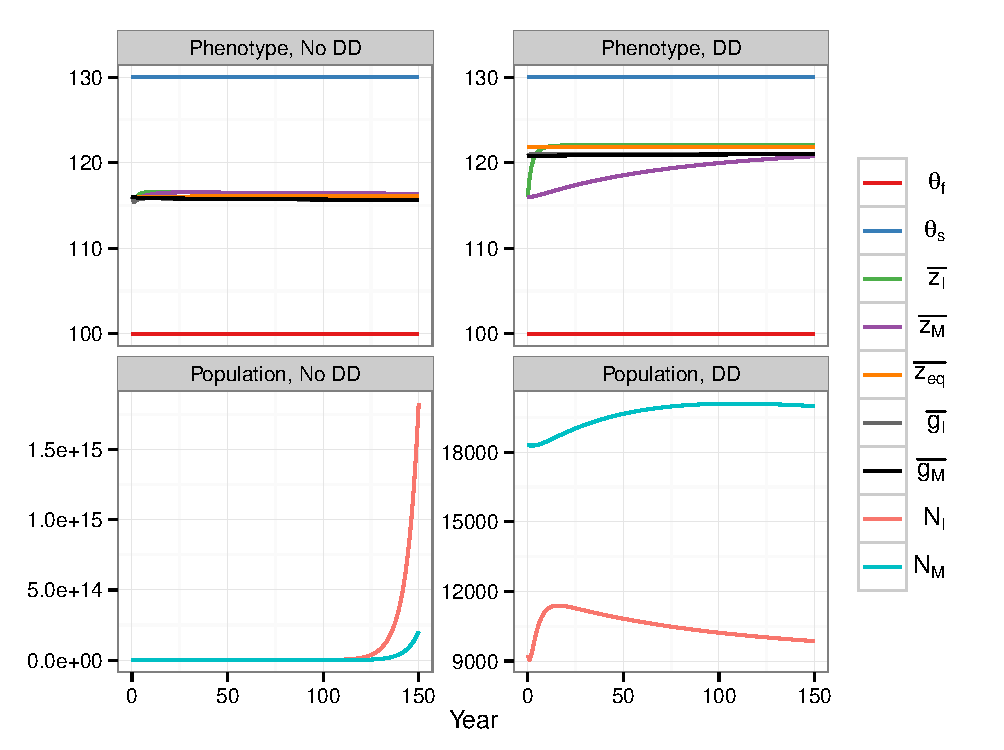
\includegraphics[scale=1]{Figures/DDphenopop.pdf}
	\caption{\textbf{Effect of density-dependence on phenotypes and populations}. \textbf{Top:} Phenotype variations in population ($\overline{z_I}, \overline{z_M}$, starting from $z = 116$) with their corresponding genotypic values ($\overline{g_I}, \overline{g_M}$, with $g_i(0) = 116$), and the approximation given by \autoref{eq:zweak}; \textbf{Bottom:} Population, number of immature individuals ($N_I$, red), number of mature individuals ($N_M$, blue). Starting from the density-dependent Stable-Stage Distribution (SSD) in constant environment. \textbf{No DD} means we used the model without density-dependence, \textbf{DD} means we implemented density-dependence through $s_0$ (see \autoref{eq:ddfunc}). Here, bud-burst date is expressed in julian days (numbered days in the year, 1st of January being 1 in julian days).}
	\label{fig:dd}
\end{figure}

We used the previously developed model in \citetext{Sandell 2014} and simulated (see~\autoref{fig:dd}) a tree population for 150 years in a constant environment, with and without density-dependence on $s_0$, to assess the effects of a more realistic demography.

As expected, density-dependence allows regulating the population (\autoref{fig:dd} right panel), as the number of mature and immature individuals seem to converge respectively to $18000$ and $10000$ individuals, while without density-dependence the population is exponentially growing.

Looking at the phenotype, we started from exactly the same starting point $z=116$ for phenotypic and genotypic values. Without density-dependence, the population quickly converge to the equilibrium phenotype ($\overline{z_{eq}}$ given by the approximation in~\autoref{eq:zweak}), $\overline{z_{eq}} = 116$ in this case. With density-dependence the equilibrium phenotype is shifted towards the survival optimum $\theta_s$ ($\overline{z_{eq}} = 121.8$). The lower seed survival $s_0$ decreases $\gamma_f$~\eqref{eq:gammaf} changing the weights in~\eqref{eq:zweak}, making it more interesting to favor the survival of already established immature trees than the production of many propagules with very little survival prospect.

The genotypic values, $\overline{g_I}$ and $\overline{g_M}$ (respectively gray and black on \autoref{fig:dd}) are distinct from the mean phenotype values.

The mean immature phenotype $\overline{z_I}$ converge quicker than the mean mature phenotype $\overline{z_M}$ to $\overline{z_{eq}}$. High mature trees survival in our simulations makes it long to replace them with a different genotype and phenotype. To make $\overline{z_M}$ closer to $\overline{z_{eq}}$, immature individuals with a phenotype closer to $\overline{z_{eq}}$ need to survive long enough to mature and outnumber initial mature individuals with phenotype further from $\overline{z_{eq}}$.

\subsection*{Fluctuating optima}

\begin{figure}[ht!]
	\centering
	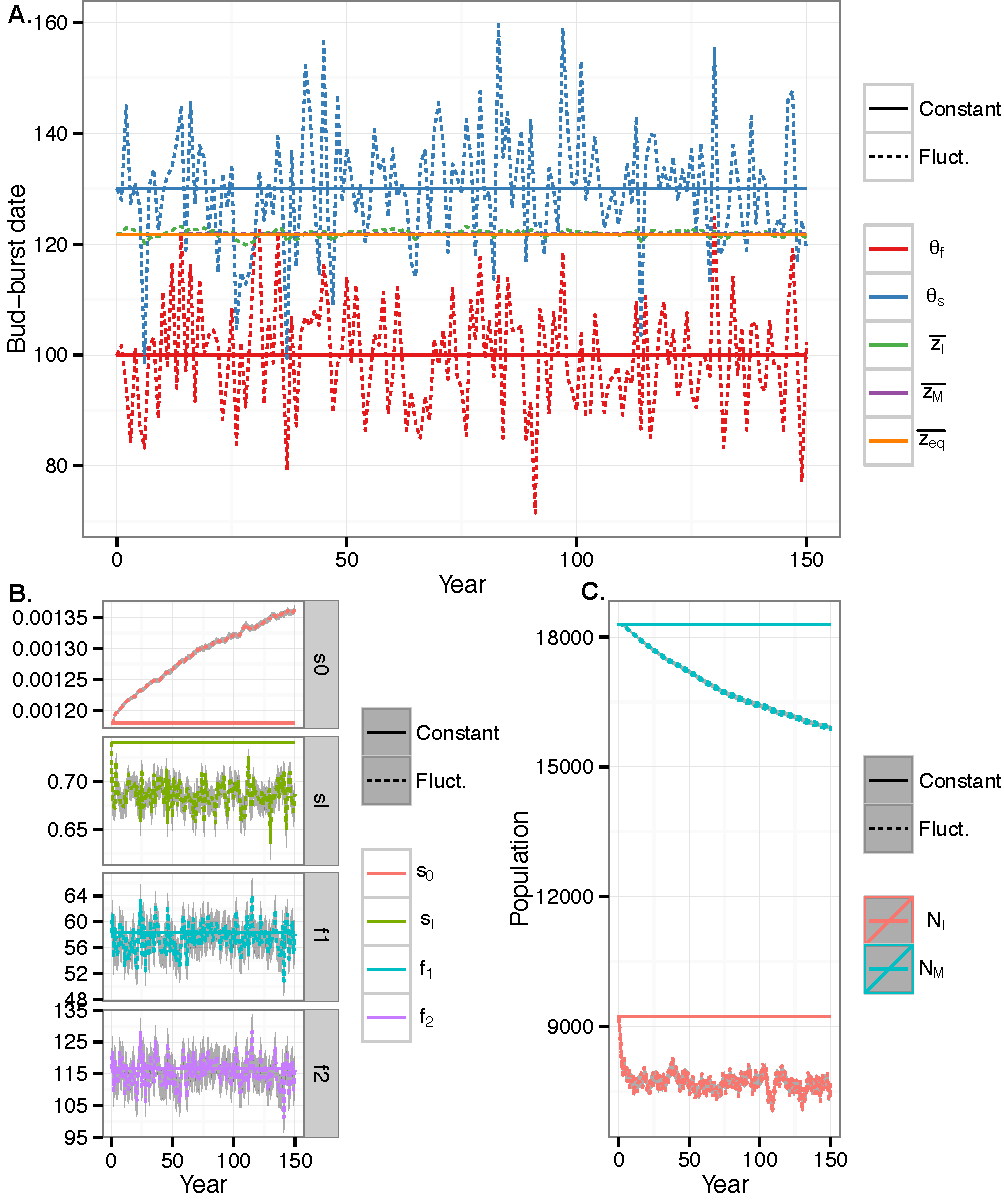
\includegraphics[scale=1]{Figures/PhenoLHTwithCorr.pdf}
	\caption{\textbf{Fluctuating optima against constant environment}. \textbf{A:} comparison of phenotypes from simulations with constant or fluctuating optima, $\overline{z_{eq}}$ is the approximation shown in \autoref{eq:zweak}; results from single simulation. \textbf{B:} life-history traits in constant or fluctuating environment. \textbf{C:} population in constant or fluctuating environment, $N_I$ is the number of immature individuals and $N_M$ the number of mature individuals, population started from the stable stage distribution. \textbf{Solid lines:} values in constant environment, \textbf{Dashed lines:} in fluctuating environment, results were averaged over 100 independent simulations. \textbf{Gray envelope}: 95\% confidence interval of average.}
	\label{fig:corr}
\end{figure}

To mimic a changing environment we made the optima fluctuate (\autoref{fig:corr}, dashed lines) and compared this model to the one in constant environment (solid lines).

The mean phenotype of the population does not change very much with the fluctuations, indeed, $\overline{z_M}$ in constant and fluctuating environment are equal, and they are also equal to $\overline{z_{eq}}$, that is why they are indistinguishable on \autoref{fig:corr}.

Only $\overline{z_I}$ fluctuates under varying environment, but the fluctuations have a very small variance compared to the ones of the optima. We found a stronger correlation between $\theta_s$ and $\overline{z_I}$ across years ($\rho_{\text{Pearson}} = 0.6997364$) than with $\theta_f$. It shows how immature individuals track the variations of the survival optimum.

Because of the variations, the phenotype lags away from the optimal value,decreasing the mean of $s_I$ in fluctuating environment. The number of immature individuals $N_I$ is thus lower under the fluctuating regime then decreasing the number of mature individuals $N_M$, this decline in density in turn increases $s_0$. The variation in $\theta_s$ causes $s_I$ to decrease, it reveals the cost of the fluctuations demographically: fluctuating regime causes variations in survival that may have dramatic effect on population.

However, those fluctuations do not seem to affect fecundities $f_1$ and $f_2$ in the same way (\autoref{fig:corr} bottom left panel). As the mean optima move, they get closer to the population phenotype increasing fecundity, but, at the next time step, they move further away from this phenotype decreasing fecundity.

The asymmetry of responses between survival $s_I$ and fecundities $f_1$ and $f_2$ is due to the specific trade-off occurring in our population. The mean phenotype in our simulations is closer to the mean of $\theta_s$ than to the mean of $\theta_f$; there is a higher chance of $\theta_s$ to be lower or much higher than the mean population phenotype when it fluctuates, while $\theta_f$ can get closer to the mean population phenotype when it fluctuates.

As we had partially correlated noises in our population (see \autoref{tab:params} to have standard parameters set), we varied correlations for noises between 0 and 1 in conditions affecting respectively survival and fecundity. The results were similar whatever the correlation coefficient. It seemed that the lower the correlation between noises, the higher were the demographic burden (results not shown). Uncorrelated environments decrease more the life-history traits than correlated environments.

\subsection*{Trend in the environment}

\begin{figure}[ht!]
	\centering
	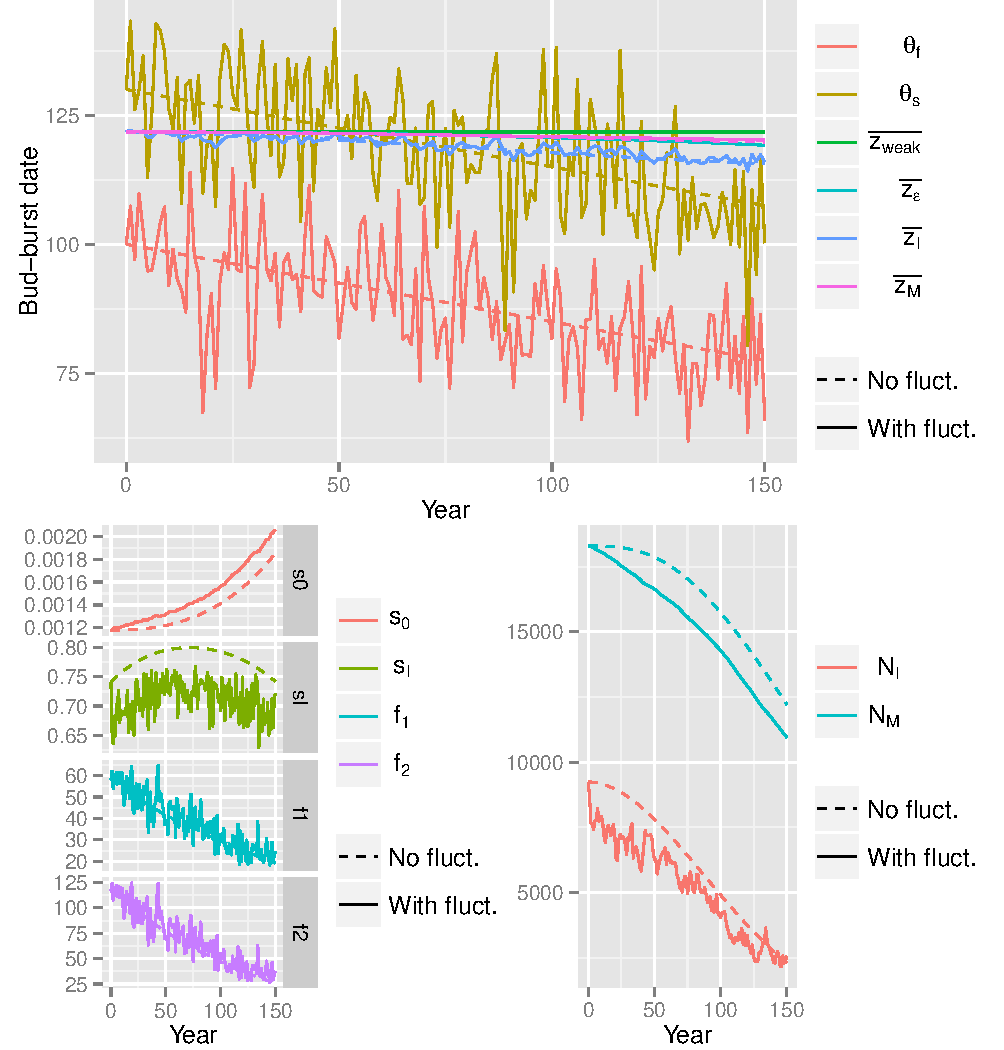
\includegraphics[scale=1]{Figures/Trend.pdf}
	\caption{\textbf{Mixed influences of trend and fluctuations on the population}. \textbf{A:} Phenotype evolution with and without fluctuations, results from a \textbf{single} simulation; \textbf{B:} (\textbf{Left}) life-history traits evolution; \textbf{C:} demography. \textbf{Solid lines:} (\textbf{No fluct.}) linearly decreasing optima with time; \textbf{Dashed lines:} (\textbf{With fluct.}) fluctuating decreasing optima, results were averaged over 100 independent simulations. \textbf{Gray envelope}: 95\% confidence interval of average.}
	\label{fig:trend}
\end{figure}

We implemented a decreasing trend in $\theta_f$ with fluctuations (\autoref{fig:trend}) to mimic climate change. We simulated both a linear trend and a linear trend with fluctuations in optima variation (respectively solid and dashed lines in \autoref{fig:trend}).

The phenotype in the population decreases as the optima decrease, but much slower, whether with fluctuations or not. The mean phenotype in the immature stage $\overline{z_I}$ varies with the same trend with and without fluctuations,  but the first still fluctuates strongly around this trend. While the mean phenotypes of mature individuals $\overline{z_M}$ are almost indistinguishable in the two types of environments, $\overline{z_M}$ under fluctuations (dashed line) is a little bit over $\overline{z_M}$ without them (solid line). We implemented the approximation $\overline{z_\epsilon}$ from (\citealt{engen_evolution_2011}, see \autoref{eq:zfluct}), it follows the variations in a similar fashion as the mean phenotype of the mature individuals.

The immature survival ($s_I$) has an interesting behavior, it first increases, reaches a maximum, then decreases. The decreasing trend in optima variation causes at first the mean population phenotype to move closer to $\theta_s$, thus maximizing $s_I$ values when it crosses $\theta_s$ line, as soon as it moves beyond $s_I$ starts to decrease again.

On the contrary $f_1$ and $f_2$ the mean population phenotype go further away from $\theta_f$ with and without fluctuation.

After a certain number of years, the population is lower in environments with trends than in constant ones, fluctuations worsen the demographic decline (\autoref{fig:trend}). 

As expected, the decreasing trend in $\theta_f$ creates a lag between the optima and the mean population values, because adaptation is slower than the rate of change. On a very long scale (2500 years), the population however maintains itself by changing its phenotype fast enough to track the optima variation with a constant lag (data not shown).

\subsection*{Estimation of the fluctuations}

\begin{figure}[ht!]
	\centering
	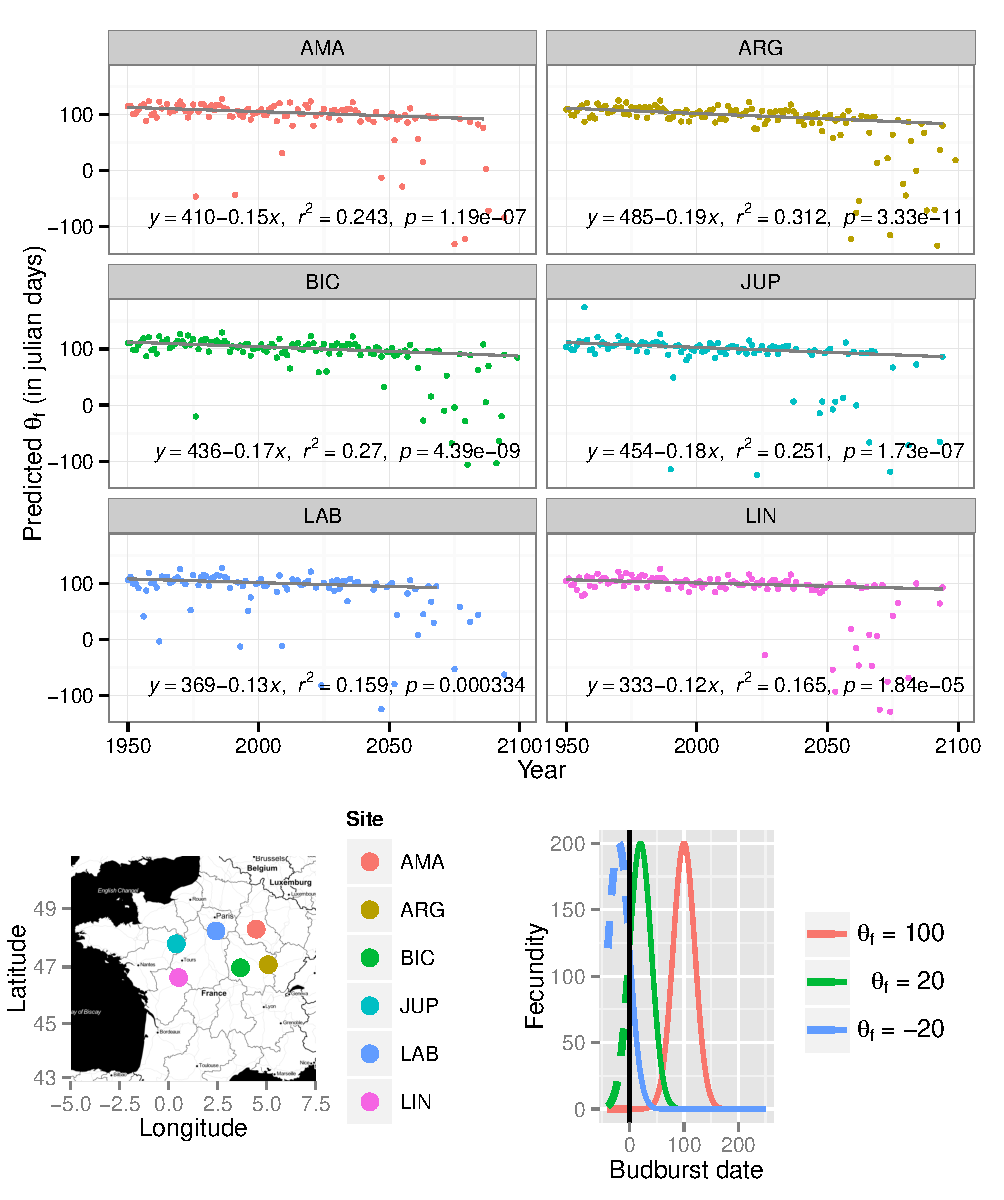
\includegraphics[scale=1]{Figures/optsmaps.pdf}
	\caption{\textbf{$\theta_{f}$ estimations from PHENOFIT data}. \textbf{A:} estimations of $\theta_f$ for each study site (see \nameref{sec:M&M} for details), linear regression only for values >60. \textbf{B:} map of the study sites. \textbf{C:} Theoretical fecundity functions with parameters from~\autoref{tab:params} with values of $\theta_f$ equals to $100$, $20$ and $-20$, solid lines indicate achievable phenotype, dashed lines advance towards previous year.}
	\label{fig:thetaf}
\end{figure}

In 6 localities (map \autoref{fig:thetaf} bottom left) using \textsc{PHENOFIT} output, we computed $\theta_f$ values at these locations (top 3 rows of \autoref{fig:thetaf}). For the 6 sites, predicted $\theta_f$ decreases with time: earlier bud-burst is favored as climate warms.

Over the general trend, we observe a small amplitude variation, corresponding to year to year change in $\theta_f$ and some more episodic dramatic decreases in its values, sometimes reaching negative values (e.g. at BIC site in 1976). The frequency of these events increase with time as they become common after 2050 for all sites. Note that those events are biased towards the decrease of $\theta_f$, as there is no equivalent dramatic increases.

The negative values of $\theta_f$ computed in \autoref{fig:thetaf}, may seem striking as negative values refer to the previous year. It indicates strong directional selection to shorten bud-burst those years. As bottom right panel of \autoref{fig:thetaf} shows, we can have negative value of $\theta_f$ and still have achievable phenotypes. If $\theta_f$ is very negative for a given year (less than -100 in 2048 for LAB), it means there will be little reproduction this year (flat tail of blue curve, bottom right panel \autoref{fig:thetaf}).

We excluded those extreme events, taking all sites together, to estimate the trend in the variation of $\theta_f$ (see~\nameref{sec:M&M}). Using linear regression on $\theta_f$ with time, we found a rate of $-0.15 \,\text{day}.\text{year}^{-1}$, with normal residuals having a variance of $93.125 \,\text{day}^2$ (data not shown, $R^2=0.2341$, $p<2\text{\sc{e}-}16$, $F=186.7$ with $611$ d.f.). From our trend model (\autoref{eq:kt}) we have:
\begin{equation}
\theta_f(t) = \overline{\theta_f} + \alpha_f k t + \alpha_f \xi_f(t).
\end{equation}
The variance of residuals is thus:
\begin{equation}
\text{Var}(\alpha_f \xi_f(t)) = \alpha_f^2 \sigma_{\xi_f}^2,
\end{equation}
which gives, with $\alpha_f = 5$, $\sigma_{\xi_f}^2 = 3.725$. Trend and variance estimations were used in previous simulations (see \autoref{tab:params}).